\documentclass[11pt]{article}
\usepackage[top=1cm, bottom=2cm, left=1cm, right=1cm]{geometry}
\usepackage{ctex}
\usepackage{float}
\usepackage{algorithm}
\usepackage{algorithmic}
\usepackage{algpseudocode}
\usepackage{amsthm,amsmath,amssymb}
\usepackage[colorlinks=true,linkcolor=blue]{hyperref}
\usepackage{listings}
\usepackage{xcolor,xparse}
\usepackage{realboxes}
\usepackage{graphics}
\usepackage{graphicx}
\usepackage{mathrsfs}
\usepackage{wrapfig}
\usepackage{subfigure}
\usepackage{pifont}

\definecolor{cmdbg}{rgb}{0.9,0.9,0.9}
\lstset{%
	basicstyle=\ttfamily,
	breaklines = true,
	backgroundcolor=\color{cmdbg},
}
\DeclareDocumentCommand{\ccmd}{v}{% 参数 v 表示工作方法类似于 \verb
    \Colorbox{cmdbg}{\csname lstinline\endcsname!#1!}%
}

\makeatletter
\newenvironment{breakablealgorithm}
  {% \begin{breakablealgorithm}
   \begin{center}
     \refstepcounter{algorithm}% New algorithm
     \hrule height.8pt depth0pt \kern2pt% \@fs@pre for \@fs@ruled
     \renewcommand{\caption}[2][\relax]{% Make a new \caption
       {\raggedright\textbf{\ALG@name~\thealgorithm} ##2\par}%
       \ifx\relax##1\relax % #1 is \relax
         \addcontentsline{loa}{algorithm}{\protect\numberline{\thealgorithm}##2}%
       \else % #1 is not \relax
         \addcontentsline{loa}{algorithm}{\protect\numberline{\thealgorithm}##1}%
       \fi
       \kern2pt\hrule\kern2pt
     }
  }{% \end{breakablealgorithm}
     \kern2pt\hrule\relax% \@fs@post for \@fs@ruled
   \end{center}
  }
\makeatother

\author{李明钰 22307110156}
\title{计算物理作业7}

\begin{document}
\maketitle


\section{题目1:单摆运动方程}
\subsection{题目描述}
Write a code to numerically solves the motion of a simple pendulum using Euler’s method, midpoint method, RK4, Euler-trapezoidal method (implement these methods by yourself). Plot the angle and total energy as a function of time. Explain the results.

\subsection{程序描述}
题目要求解一个简谐摆\ref{fig:简谐摆受力示意图}的运动,其运动所满足的偏微分方程为
\begin{equation}
    \frac{d^2 \theta}{d t^2} + \frac{g}{L} \sin{\theta} = 0 \qquad 
    \theta|_{t=0} = \theta_0 \qquad \frac{d \theta}{d t}|_{t=0}=0
\end{equation}
令$\omega = \frac{d\theta}{dt}$,上述二阶微分方程可以被转化为两个一阶微分方程所组成的方程组。
\begin{equation}
\begin{aligned}
\frac{d\omega}{dt}&=-\frac{g}{L}\sin{\theta}\\
\frac{d\theta}{dt}&=\omega\\
\omega|_{t=0}=\omega_0 &\qquad \theta|_{t=0}=\theta_0
\end{aligned}
\end{equation}
\begin{figure}[h]
    \centering
    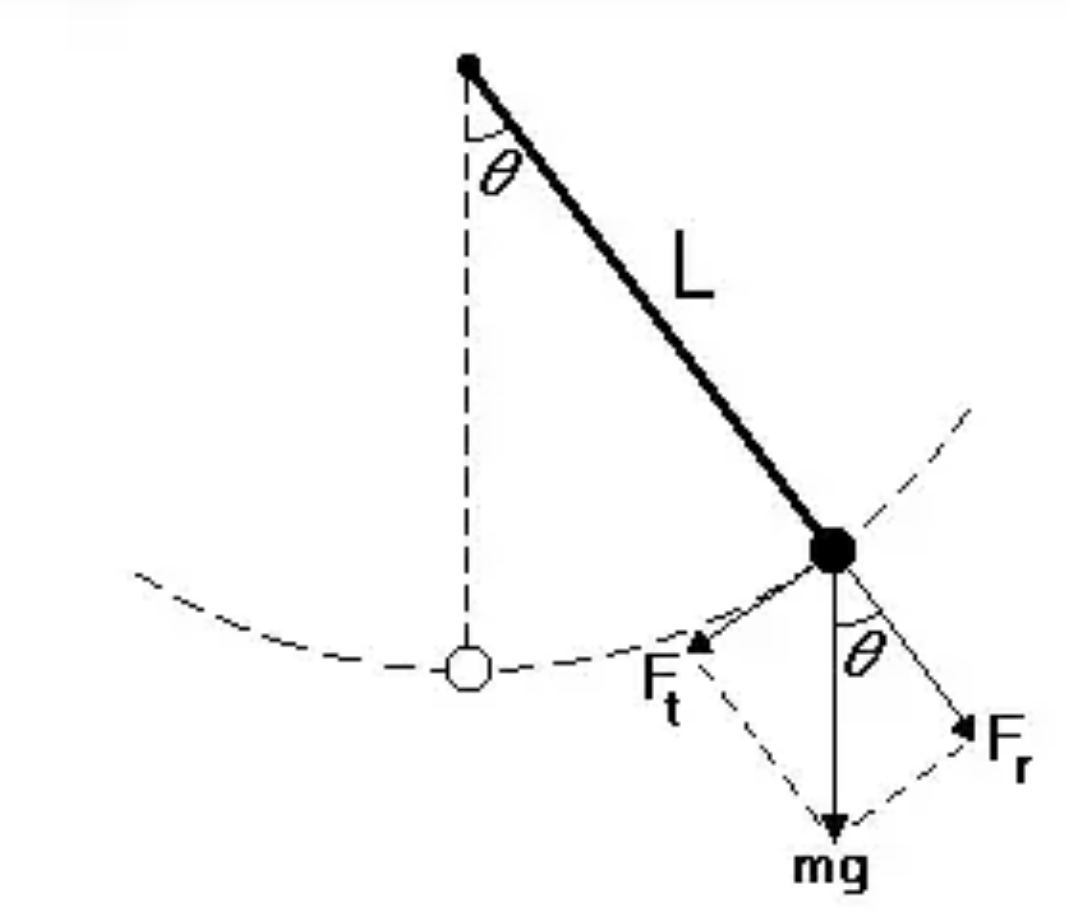
\includegraphics[width=0.3\linewidth]{简谐摆受力示意图.png}
    \caption{简谐摆受力示意图}
    \label{fig:简谐摆受力示意图}
\end{figure}
\subsection{伪代码}
PS:这里因为Latex的algorithm包和algpseudocode包之间的冲突末尾多了一个0,但是不影响阅读
\begin{breakablealgorithm}

\caption{Euler Method}
\label{Euler Method}
\begin{algorithmic}[1]
\REQUIRE  $\theta_0$, $\omega_0$  $t\in \mathrm{R}^n$
\ENSURE $\theta(t)$,$E(t)$ 
\STATE $\Delta t \gets \text{diff}(t)$

\STATE $\theta[0] \gets \theta_0$
\STATE $\omega[0] \gets \omega_0$

\FOR{$i = 1$ to $n-1$}
    \STATE $h \gets \Delta t[i-1]$
    \STATE $\omega[i] \gets \omega[i-1] - h \cdot \frac{g}{L} \cdot \sin(\theta[i-1])$
    \STATE $\theta[i] \gets \theta[i-1] + h \cdot \omega[i-1]$
\ENDFOR

\STATE $E \gets -m \cdot g \cdot L \cdot \cos(\theta) + 0.5 \cdot m \cdot (L \cdot \omega)^2$

\RETURN $\theta(t), E(t)$
\end{algorithmic}
    
\end{breakablealgorithm}

\begin{breakablealgorithm}

\caption{Midpoint Method}
\label{Midpoint Method}
\begin{algorithmic}[1]
\REQUIRE Initial conditions $\theta_0$, $\omega_0$, time array $t$, constants $g$, $L$, $m$
\STATE $n \gets \text{length of } t$
\STATE $\Delta t \gets \text{array of time steps (computed as } t[i+1] - t[i] \text{)}$
\STATE Initialize arrays: $\theta, \omega, \Delta_\theta, \Delta_\omega \gets \text{zeros of size } n$
\STATE $\theta[0] \gets \theta_0$, $\omega[0] \gets \omega_0$

\FOR{$i \gets 1$ to $n-1$}
    \STATE $h \gets \Delta t[i-1]$
    \STATE $\Delta_\omega[i-1] \gets h \cdot \left(-\frac{g}{L} \sin(\theta[i-1])\right)$
    \STATE $\Delta_\theta[i-1] \gets h \cdot \omega[i-1]$
    \STATE $\omega[i] \gets \omega[i-1] + h \cdot \left(-\frac{g}{L} \sin\left(\theta[i-1] + 0.5 \cdot \Delta_\theta[i-1]\right)\right)$
    \STATE $\theta[i] \gets \theta[i-1] + h \cdot \left(\omega[i-1] + 0.5 \cdot \Delta_\omega[i-1]\right)$
\ENDFOR

\STATE $E \gets -m \cdot g \cdot L \cdot \cos(\theta) + 0.5 \cdot m \cdot (L \cdot \omega)^2$
\RETURN $\theta, E$
\end{algorithmic}

\end{breakablealgorithm}
\begin{breakablealgorithm}

\caption{RK4}\label{RK4}
    \begin{algorithmic}[1]
\REQUIRE Initial conditions $\theta_0$, $\omega_0$, time array $t$, constants $g$, $L$, $m$
\STATE $n \gets \text{length of } t$
\STATE $\Delta t \gets \text{array of time steps (computed as } t[i+1] - t[i] \text{)}$
\STATE Initialize arrays: $\theta, \omega \gets \text{zeros of size } n$
\STATE $\theta[0] \gets \theta_0$, $\omega[0] \gets \omega_0$

\FOR{$i \gets 1$ to $n-1$}
    \STATE $h \gets \Delta t[i-1]$
    \STATE $K_1^\theta \gets \omega[i-1]$
    \STATE $K_1^\omega \gets -\frac{g}{L} \sin(\theta[i-1])$
    
    \STATE $K_2^\theta \gets \omega[i-1] + 0.5 \cdot h \cdot K_1^\omega$
    \STATE $K_2^\omega \gets -\frac{g}{L} \sin\left(\theta[i-1] + 0.5 \cdot h \cdot K_1^\theta\right)$
    
    \STATE $K_3^\theta \gets \omega[i-1] + 0.5 \cdot h \cdot K_2^\omega$
    \STATE $K_3^\omega \gets -\frac{g}{L} \sin\left(\theta[i-1] + 0.5 \cdot h \cdot K_2^\theta\right)$
    
    \STATE $K_4^\theta \gets \omega[i-1] + h \cdot K_3^\omega$
    \STATE $K_4^\omega \gets -\frac{g}{L} \sin\left(\theta[i-1] + h \cdot K_3^\theta\right)$
    
    \STATE $\theta[i] \gets \theta[i-1] + \frac{h}{6} \cdot \left(K_1^\theta + 2 \cdot K_2^\theta + 2 \cdot K_3^\theta + K_4^\theta\right)$
    \STATE $\omega[i] \gets \omega[i-1] + \frac{h}{6} \cdot \left(K_1^\omega + 2 \cdot K_2^\omega + 2 \cdot K_3^\omega + K_4^\omega\right)$
\ENDFOR

\STATE $E \gets -m \cdot g \cdot L \cdot \cos(\theta) + 0.5 \cdot m \cdot (L \cdot \omega)^2$
\RETURN $\theta, E$
\end{algorithmic}
\end{breakablealgorithm}
\begin{breakablealgorithm}
    
\caption{EulerTrapezoidalMethod}\label{EulerTrapezoidalMethod}
\begin{algorithmic}[1]
\REQUIRE Initial conditions $\theta_0$, $\omega_0$, time array $t$, constants $g$, $L$, $m$, tolerance $\epsilon$
\STATE $n \gets \text{length of } t$
\STATE $\Delta t \gets \text{array of time steps (computed as } t[i+1] - t[i] \text{)}$
\STATE Initialize arrays: $\theta, \omega \gets \text{zeros of size } n$
\STATE $\theta[0] \gets \theta_0$, $\omega[0] \gets \omega_0$

\FOR{$i \gets 1$ to $n-1$}
    \STATE $h \gets \Delta t[i-1]$
    
    \STATE \textbf{Euler Prediction:}
    \STATE $\omega_\text{Euler} \gets \omega[i-1] + h \cdot \left(-\frac{g}{L} \sin(\theta[i-1])\right)$
    \STATE $\theta_\text{Euler} \gets \theta[i-1] + h \cdot \omega[i-1]$
    
    \STATE \textbf{First Correction:}
    \STATE $\omega^\text{correct}_0 \gets \omega[i-1] + \frac{h}{2} \cdot \left(\left(-\frac{g}{L} \sin(\theta[i-1])\right) + \left(-\frac{g}{L} \sin(\theta_\text{Euler})\right)\right)$
    \STATE $\theta^\text{correct}_0 \gets \theta[i-1] + \frac{h}{2} \cdot \left(\omega[i-1] + \omega_\text{Euler}\right)$
    
    \STATE $\omega^\text{correct}_1 \gets \omega[i-1] + \frac{h}{2} \cdot \left(\left(-\frac{g}{L} \sin(\theta^\text{correct}_0)\right) + \left(-\frac{g}{L} \sin(\theta[i-1])\right)\right)$
    \STATE $\theta^\text{correct}_1 \gets \theta[i-1] + \frac{h}{2} \cdot \left(\omega[i-1] + \omega^\text{correct}_0\right)$
    
    \STATE \textbf{Iterative Refinement:}
    \WHILE{$\left|\omega^\text{correct}_0 - \omega^\text{correct}_1\right| > \epsilon$ \OR $\left|\theta^\text{correct}_0 - \theta^\text{correct}_1\right| > \epsilon$}
        \STATE $\omega^\text{correct}_0 \gets \omega^\text{correct}_1$
        \STATE $\theta^\text{correct}_0 \gets \theta^\text{correct}_1$
        \STATE $\omega^\text{correct}_1 \gets \omega[i-1] + \frac{h}{2} \cdot \left(\left(-\frac{g}{L} \sin(\theta^\text{correct}_0)\right) + \left(-\frac{g}{L} \sin(\theta[i-1])\right)\right)$
        \STATE $\theta^\text{correct}_1 \gets \theta[i-1] + \frac{h}{2} \cdot \left(\omega[i-1] + \omega^\text{correct}_0\right)$
    \ENDWHILE
    
    \STATE $\theta[i] \gets \theta^\text{correct}_0$
    \STATE $\omega[i] \gets \omega^\text{correct}_0$
\ENDFOR

\STATE $E \gets -m \cdot g \cdot L \cdot \cos(\theta) + 0.5 \cdot m \cdot (L \cdot \omega)^2$
\RETURN $\theta, E$
\end{algorithmic}
\end{breakablealgorithm}
\subsection{输入输出实例}
初始条件设为最常见的
\begin{equation}
    \begin{aligned}
        \theta|_{t=0}=\frac{\pi}{2} \qquad \omega|_{t=0} = 0
    \end{aligned}
\end{equation}
用不同算法解得的$\theta(t)$(图\ref{fig:不同算法解得的theta})和$E(t)$(图\ref{fig:不同算法解得的E}),可以发现欧拉法的计算得到的能量较快发散,而其他算法发散的很慢。
\begin{figure}[h]
    \centering
    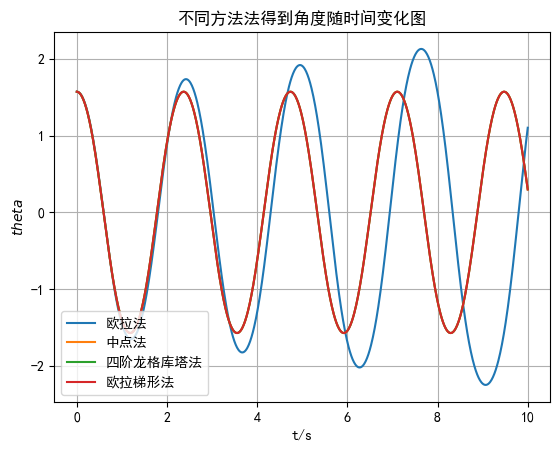
\includegraphics[width=0.5\linewidth]{t1_theta.png}
    \caption{不同算法解得的$\theta(t)$}
    \label{fig:不同算法解得的theta}
\end{figure}

\begin{figure}
    \centering
    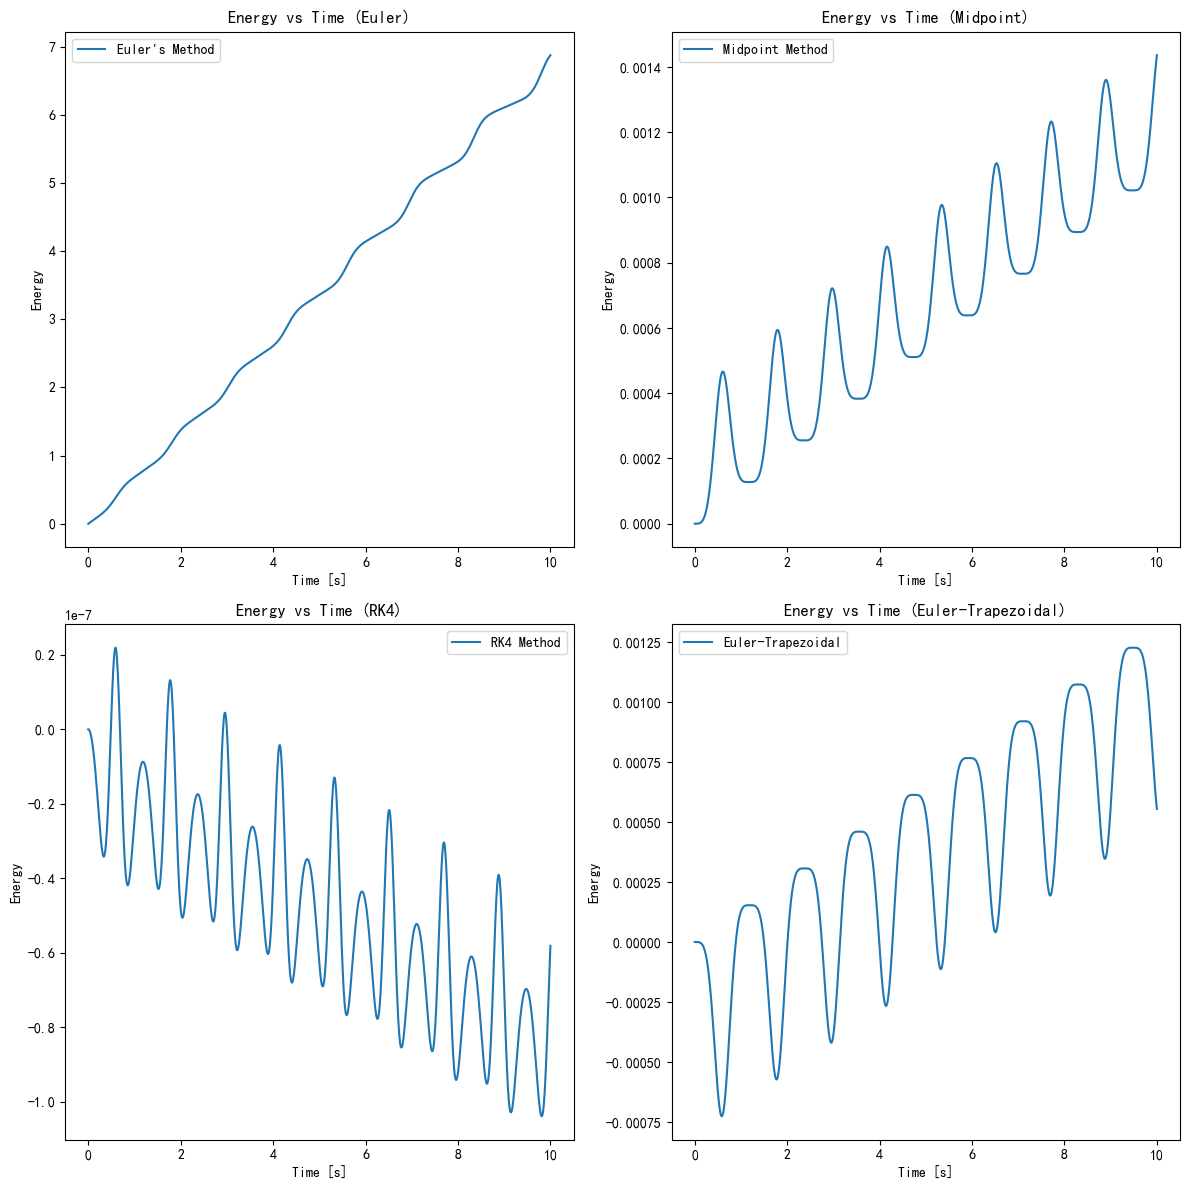
\includegraphics[width=0.5\linewidth]{t1_E.png}
    \caption{不同算法解得的$E(t)$}
    \label{fig:不同算法解得的E}
\end{figure}
\subsection{对现象的解释}
所有的算法都会有一个误差最终导致发散,这一发散速度与算法的误差量级有关,其中欧拉法(算法\ref{Euler Method})的全局误差$\propto O(h)$,而中点法(算法\ref{Midpoint Method})全局误差$\propto O(h^2)$,四阶龙格-库塔方法(算法\ref{RK4})全局误差$\propto O(h^4)$,而欧拉梯形法则(算法\ref{EulerTrapezoidalMethod})的误差则只与我们设置的可允许误差$\epsilon$有关,其全局误差$\propto O(\epsilon)$,但是此误差不是单向误差不容易堆积,因此其结果发散速度也很慢。

\section{题目2:氢原子和锂原子的薛定谔方程}
\subsection{题目描述}
Write a code to numerically solves radial Schrödinger equation for
\begin{equation}
    \[
\left[-\frac{1}{2}\nabla^2 + V(\mathbf{r})\right]\psi(\mathbf{r}) = E\psi(\mathbf{r}), \quad V(\mathbf{r}) = V(\mathbf{r})
\]
\end{equation}
(1)V(r) = -1/r(hydrogen atom)
(2)V(r) = -\frac{Z_{ion}}{}
\subsection{程序描述}
适用有限差分法(算法\ref{Finite Difference Method for Solving Radial Schrödinger Equation})分别解氢原子和锂原子的薛定谔方程,并输出能量最低的三个本征能量。
\subsection{伪代码}
PS:这里因为Latex的algorithm包和algpseudocode包之间的冲突行号全部变为0且末尾多了一个0,但是不影响阅读
\begin{breakablealgorithm}
    

\caption{Finite Difference Method for Solving Radial Schrödinger Equation}
\label{Finite Difference Method for Solving Radial Schrödinger Equation}
\begin{algorithmic}[1]
\State \textbf{Input:} Potential function \texttt{potential\_function}
\State \textbf{Output:} Eigenvalues and Eigenvectors

\State $r_{\text{min}} \gets 1$ \Comment{Initial radius (avoid singularity at r=0)}
\State $num\_points \gets 2000$ \Comment{Number of grid points}
\State $t_{\text{max}} \gets \ln(40)$ \Comment{Transformed time range}
\State $dt \gets \frac{t_{\text{max}}}{num\_points}$ \Comment{Time step size}
\State $t\_values \gets \text{linspace}(dt, t_{\text{max}}, num\_points)$

\State $r\_values \gets r_{\text{min}} \cdot (\exp(t\_values) - 1)$ \Comment{Generate radial grid points via transformation}
\State $eigenvalues \gets []$ \Comment{List to store eigenvalues}
\State $eigenvectors \gets []$ \Comment{List to store eigenvectors}

\For{angular\_momentum = 0, 1, 2} \Comment{For each angular momentum quantum number l = 0, 1, 2}
    \State $hamiltonian \gets \text{zeros}(num\_points, num\_points)$ \Comment{Construct Hamiltonian matrix}
    \State $potential\_values \gets \text{potential\_function}(r\_values)$

    \For{$i = 0$ to $num\_points-1$}
        \State $scaling\_factor \gets \frac{1}{(r_{\text{min}} \cdot \exp(t\_values[i]))^2} \div 2$
        \State $hamiltonian[i, i] \gets potential\_values[i] + \frac{angular\_momentum \cdot (angular\_momentum + 1)}{r\_values[i]^2} + \frac{2}{dt^2} \cdot scaling\_factor$
        \If{$i < num\_points - 1$}
            \State $hamiltonian[i, i+1] \gets -\frac{1}{dt^2} \cdot scaling\_factor + \frac{1}{2dt} \cdot scaling\_factor$
        \EndIf
        \If{$i > 0$}
            \State $hamiltonian[i, i-1] \gets -\frac{1}{dt^2} \cdot scaling\_factor - \frac{1}{2dt} \cdot scaling\_factor$
        \EndIf
    \EndFor

    \State $eigvals, eigvecs \gets \text{eig}(hamiltonian)$ \Comment{Solve for eigenvalues and eigenvectors}
    \State $sorted\_indices \gets \text{argsort}(eigvals)$ \Comment{Sort eigenvalues}
    \For{$idx$ in $sorted\_indices[0:3]$} \Comment{Take the first 3 smallest eigenvalues}
        \State $eigenvalues.append([eigvals[idx], angular\_momentum, angular\_momentum + idx + 1])$
        \State $eigenvectors.append(eigvecs[:, idx])$
    \EndFor
\EndFor

\State $eigenvalues \gets \text{array}(eigenvalues)$
\State $lowest\_indices \gets \text{argsort}(eigenvalues[:, 0])[0:3]$ \Comment{Get indices of the three lowest energy eigenvalues}
\end{algorithmic}
\end{breakablealgorithm}
\subsection{输入输出实例}
计算得到结果如下:

\begin{figure}[h]
    \centering
    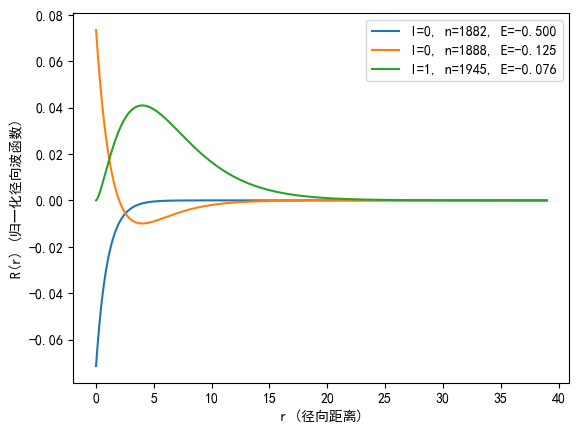
\includegraphics[width=0.5\linewidth]{氢原子R.png}
    \caption{氢原子能量最低的三个本征态R(r)}
    \label{fig:my_label}
\end{figure}

\begin{figure}
    \centering
    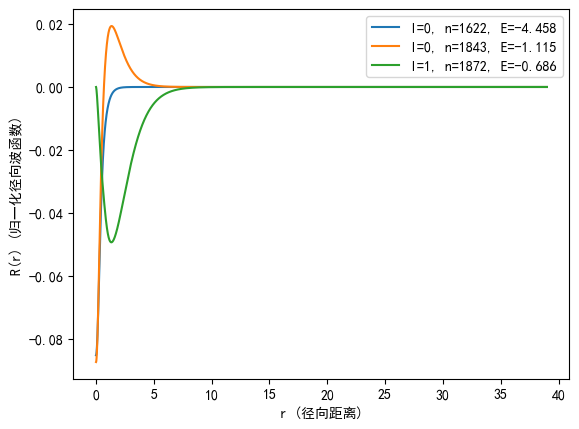
\includegraphics[width=0.5\linewidth]{锂原子R.png}
    \caption{锂原子能量最低的三个本征态R(r)}
    \label{fig:my_label}
\end{figure}
\end{document}
